\documentclass[spanish]{article}
\usepackage{amsmath, amsfonts, amsthm}
\usepackage{float}
\usepackage{tikz}
\usetikzlibrary{automata, arrows, arrows.meta, positioning, babel, shapes.misc}
\tikzset{shorten >= 1pt,
         node distance = 2cm, on grid,
         >= stealth,
         every initial
           by arrow/.style = -{Straight Barb[length = 1.1ex]},
         initial text = {},
         initial distance = 0.05,
         every state/.style = {minimum size = 5mm},
         bend angle = 20,
         every loop/.style = {looseness = 13}}

\newcommand{\tnum}{2}
\begin{document}

\title{
    Tarea 2 \\
    Informática Teórica
}
\author{
    Matías Peñaloza
    202373037-8
}
\date{
    2024-2
}
\maketitle

\begin{center}
  \begin{tabular}{|l|r|}
    \hline
    \multicolumn{1}{|c|}{\textbf{Concepto}} &
      \multicolumn{1}{c|}{\textbf{Tiempo [min]}} \\
    \hline
    Revisión & 60\\
    \hline
    Desarrollo    & 90\\
    \hline
    Informe	      & 90\\
    \hline
  \end{tabular}
\end{center}

\section{Enunciado}
\begin{enumerate}
  \item % 20242t1p1
    Describa concisamente el lenguaje aceptado por el autómata
    de la figura 1.
    \begin{figure}[ht]
      \centering
      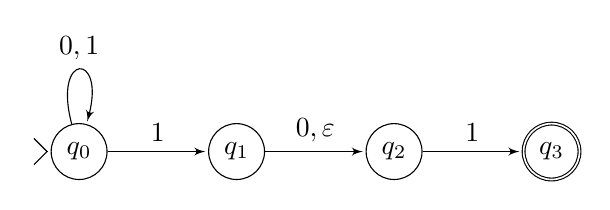
\begin{tikzpicture}
        \node[state, initial]	       (q0)		     {\(q_0\)};
        \node[state]		       (q1) [right of = q0]  {\(q_1\)};
        \node[state]		       (q2) [right of = q1]  {\(q_2\)};
        \node[state, accepting]	       (q3) [right of = q2]  {\(q_3\)};

        \path[-latex'] (q0) edge [loop above] node {\(0, 1\)}	      (q0);
        \path[-latex'] (q0) edge node[above] {\(1\)}		      (q1);
        \path[-latex'] (q1) edge node[above] {\(0, \varepsilon\)}     (q2);
        \path[-latex'] (q2) edge node[above] {\(1\)}		      (q3);
      \end{tikzpicture}
      \caption{Un autómata finito}
      \label{fig:20242t2p1}
    \end{figure}
    \hspace*{\fill}(40 puntos)
  \item % 20242t2p2
    Construya un DFA lo más simple posible
    que reconozca el lenguaje aceptado
    por el autómata de la figura 1.
    \\ \hspace*{\fill}(60 puntos)
  \end{enumerate}
  
\section{Desarrollo}
	\subsection{Lenguaje aceptado por el autómata}
    	Para describir el lenguaje aceptado por el autómata utilizaremos expresiones regulares.\\Escribiremos las expresiones regulares que nos llevan del estado $q_{i}$ al $q_{i+1}$, con las cuales podremos armar la expresión regular que nos llevará de $q_0$ a $q_n$.\\\\
        Ahora, para el estado $q_0$ podemos ver que podemos llegar a él con:
        $$\varepsilon, 0, 1$$
        Luego 0 y 1 son parte de un bucle, teniendo eso en cuenta la expresión regular que nos lleva al primer estado $q_0$ sería:
        $$(0|1)^*$$
       	Para llegar al estado $q_1$ únicamente tenemos:
        $$1$$
        por lo que este mismo símbolo sería la expresión regular que nos lleva de $q_0$ a $q_1$.\\\\
        Para llegar al estado $q_2$ tenemos:
        $$0, \varepsilon$$
        de los cuales ninguno forma parte de un bucle, lo que nos lleva a la siguiente expresión:
        $$(0|\varepsilon)$$
        la cual nos lleva del estado $q_1$ al $q_2$.\\\\
        Para llegar al estado final $q_3$ únicamente tenemos:
        $$1$$
        por lo que este mismo símbolo representa la expresión regular que nos lleva de $q_2$ al estado final $q_3$.\\\\
        Finalmente, la expresión regular que describe el lenguaje aceptado por el autómata es:
        $$(0|1)^*1(0|\varepsilon)1$$
        
    \subsection{DFA mínimo}
        Podemos identificar que el autómata de la figura es un NFA, por lo que primero lo convertiremos en un DFA utilizando $\varepsilon$-closure.
        Notar que los únicos conjuntos que serán distintos de sí mismos al aplicar $\varepsilon$-closure son aquellos que contienen al estado $q_1$, ya que:
        \begin{center}
          $\varepsilon$-closure($\{q_0\}$) $= \{q_0\}$\\
          $\varepsilon$-closure($\{q_1\}$) $= \{q_1, q_2\}$\\
          $\varepsilon$-closure($\{q_2\}$) $= \{q_2\}$\\
          $\varepsilon$-closure($\{q_3\}$) $= \{q_3\}$
        \end{center}
        Una vez dicho esto, armamos la tabla del algoritmo:
          \begin{table}[H]
            \centering
            \begin{tabular}{|c|c|c|c|c|c|}
              \hline
              Tag & conjunto & $\varepsilon$-closure & 0 & 1 & Tipo \\ 
              \hline
              A & $\{q_0\}$ & $\{q_0\}$ & A & B & Inicial\\
              \hline
              B & $\{q_0,q_1\}$ & $\{q_0,q_1,q_2\}$ & C & D & Intermedio\\ 
              \hline
              C & $\{q_0,q_2\}$ & $\{q_0,q_2\}$ & A & D & Intermedio\\
              \hline
              D & $\{q_0,q_1,q_3\}$ & $\{q_0,q_1,q_2,q_3\}$ & C & D & Final\\
              \hline
            \end{tabular}
          \end{table}
        \\
        Ahora, a partir de la tabla armaremos nuestro DFA:\\
          \begin{figure}[H]
            \centering
            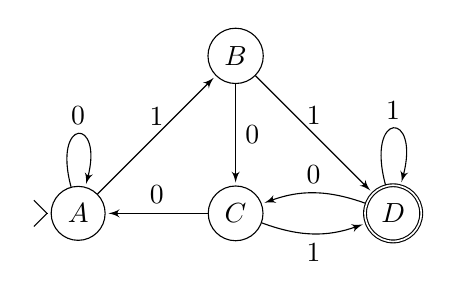
\begin{tikzpicture}
              \node[state, initial]	       (A)		     {\(A\)};
              \node[state]		       (C) [right of = A]  {\(C\)};
              \node[state]		       (B) [above of = C]  {\(B\)};
              \node[state, accepting]	       (D) [right of = C]  {\(D\)};
      
              \path[-latex'] (A) edge [loop above] node {\(0\)}	      (A);
              \path[-latex'] (A) edge node[above] {\(1\)}		          (B);
              \path[-latex'] (B) edge node[right] {\(0\)}             (C);
              \path[-latex'] (B) edge node[above] {\(1\)}             (D);
              \path[-latex'] (C) edge node[above] {\(0\)}		          (A);
              \path[-latex'] (C) edge[bend right] node[below] {\(1\)}		          (D);
              \path[-latex'] (D) edge [loop above] node {\(1\)}	      (D);
              \path[-latex'] (D) edge[bend right] node[above] {\(0\)}		          (C);
  
            \end{tikzpicture}
            \caption{DFA}
          \end{figure}
          Ahora utilizaremos el algoritmo de Moore para encontrar el DFA mínimo, por lo que procedemos
          a hacer la tabla de transición del DFA encontrado:\\
          \begin{table}[H]
              \centering
              \begin{tabular}{|c c|c|c|}
                  \hline
                  Grupo & \space & 0 & 1\\
                  \hline
                  \space & A & Q & Q\\
                  No final Q & B & Q & F\\
                  & C & Q & F\\
                  \hline
                  Final F & D & Q & F\\
                  \hline
              \end{tabular}
          \end{table}
          
          Luego dividimos Q:\\
          
          \begin{table}[H]
              \centering
              \begin{tabular}{|c c|c|c|}
                  \hline
                  Grupo & \space & 0 & 1\\
                  \hline
                  Q$_1$ & A & Q$_1$ & Q$_2$\\
                  \hline
                  Q$_2$ & B & Q$_2$ & F\\
                  \space & C & Q$_1$ & F\\
                  \hline
                  F & D & Q$_2$ & F\\
                  \hline
              \end{tabular}
          \end{table}
          
          En este punto, podemos ver que al dividir Q$_2$ obtendremos los mismos estados y, por lo tanto, el mismo DFA.
          Así que concluimos que el DFA de la figura 2 es el DFA mínimo y, por lo tanto, el más simple.
          

\end{document}
